
\section{Experimentation}
\label{sec:experimentation}

% \TODO{Define what we want.} We measure the time between the broadcast of a
% message and its delivery by all processes in the network. We expect that our
% measurements slowly increase as the network becomes more dynamic.

\begin{figure*}
  \begin{center}
    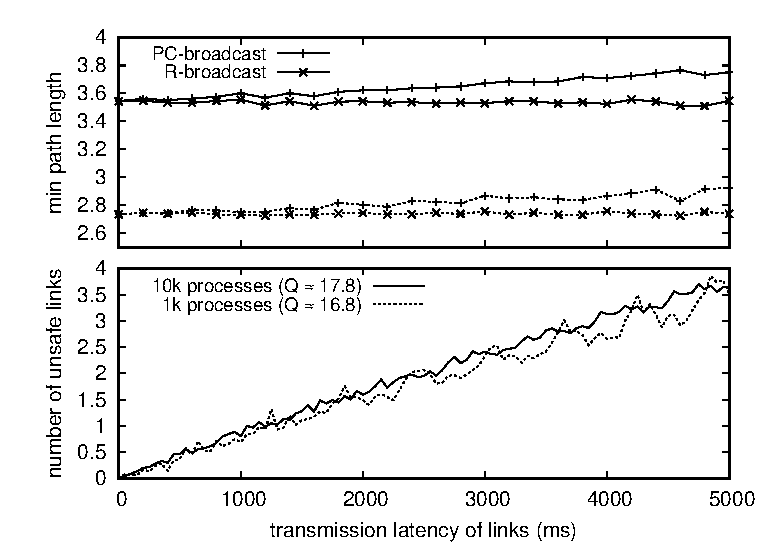
\includegraphics[width=1.5\columnwidth]{./img/delay.eps}
    \caption{\label{fig:delay}Impact of \CBROADCAST on the underlying overlay
      network.}
  \end{center}
\end{figure*}

\CBROADCAST provides causal order with constant size message
overhead. This feature comes at a cost: at first, new communication
means are disable for causal broadcast. In this section, we evaluate
the impact of \CBROADCAST on the message delivery in a specific
overlay network that corresponds to random graphs. The experiments run
on the \PEERSIM simulator~\cite{montresor2009peersim} that allows
simulations to reach high scale in terms of number of processes. Our
implementation is available on the Github platform at
\url{http://github.com/chat-wane/peersim-pcbroadcast}.


\noindent \textbf{Objective:} To observe the transmission delay introduced by
\CBROADCAST on message delivery. We expect the delay to increase as the latency
increase.

\noindent \textbf{Description:} We build an overlay network with a topology
close to random graphs using \SPRAY~\cite{nedelec2017adaptive}. The overlay
networks comprises 1k, and 10k processes. Networks are dynamic. Each process'
neighborhood $Q$ changes at least once every 60 seconds; and on average twice
every 60 seconds. Each exchange involves two processes that both add and remove
half of their partial view.  Links are FIFO, bidirectional, and have
transmission delays. The delay increases over time up to 5 seconds.
Consequently, the duration of ping phases increases during the experiment.
Links become safe slower. \\
We measure the shortest path length from a random set of processes to all other
processes. It represents the average number of hops taken by broadcast messages
before being received and delivered by all processes. Multiplied by the
transmission latency of links, it represents the transmission delay of broadcast
messages before being received by all processes. \\
We perform measurements on 2 broadcast protocols: \CBROADCAST and R-broadcast.
R-broadcast uses all available links to broadcast messages in a gossip fashion.
Transmission delays before delivery are similar to piggybacking approaches~\cite{almeida2008interval,fidge1988timestamps,mattern1989virtual,singhal1992efficient}~\cite{birman1987reliable,hadzilacos1993fault,mostefaoui2017probabilistic} without accounting for the time taken to send large messages (e.g. each
message convey a vector clock of 10k entries when the network comprises 10k
processes).  Larger packets induces larger transmission time.

\noindent \textbf{Results:} Figure~\ref{fig:delay} shows the result of the
experiment. The y-axis depicts the delay set on message transmission for each
link. The top part of the figure shows the average shortest path length. The
bottom part of the figure shows the average number of unsafe links per process
that cannot be used for causal broadcast yet.
\begin{itemize}[leftmargin=*]
\item Figure~\ref{fig:delay} shows that both R-broadcast and \CBROADCAST deliver
  message quickly to all processes. The overlay network guarantee that paths
  stay short and logarithmically scaling with the number of random neighbors in
  partial views.
\item The top part of Figure~\ref{fig:delay} shows that measurements made on
  \CBROADCAST increases while measurements made on R-broadcast stay
  constant. R-broadcast uses all neighbors provided by \SPRAY while \CBROADCAST
  excludes links still in buffering phase. The more latency on transmission, the
  longer the buffering phase. The bottom part of Figure~\ref{fig:delay} shows
  that the number of elements in the buffers increases accordingly.
\item Figure~\ref{fig:delay} shows that the growth of path length stays small
  even when transmission delays become high. The number of elements in buffers
  stays small because the buffering phase takes a constant number of hops to
  complete: at most 3 hops. The path length grows even slower, for removing 3
  among 17 links has restricted impact on overlay networks close to random
  graphs.
\end{itemize}

This experimentation shows that even under bad network conditions (high
transmission delays) and using highly dynamic overlay networks (random
peer-sampling), the number of unsafe links remains small. The negative impact
expected on transmission time before message delivery remains small. In
practice, we expect smaller network transmission delays, and overlay networks
less subject to neighborhood changes (e.g. exploiting user preferences, or
geolocalisation). In such settings, we expect \CBROADCAST to have a negligible
negative impact on the overlay network properties.

The next section reviews state-of-the-art techniques designed to maintain causal
order among messages.

%%% Local Variables:
%%% mode: latex
%%% TeX-master: "../paper"
%%% End:
